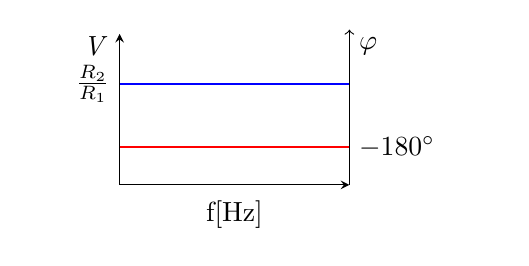
\begin{tikzpicture}[scale=1, transform shape]
    \begin{axis}[
        width=4.5cm, % Breite des Graphen
        height=3.5cm, % Höhe des Graphen
        xmin=0, xmax=10,
        ymin=0, ymax=120,
        axis lines=left,
        axis on top=true,
        domain=0:10,
        xtick=\empty,
        ytick=\empty,
        ylabel style={rotate=270, anchor=east, yshift=0.8cm},
         ylabel={\it V},
        xlabel={f[Hz]},
        clip mode=individual % Verhindert das Abschneiden von Elementen
        ]
        \path[draw=none] (axis cs:-4, 0) rectangle (axis cs:16.6,120);
    
        \addplot+[mark=none, thick, blue] coordinates {(0,80) (10,80)};
        % Adding the left-side label
        \node[anchor=east] at (axis cs:0,80) {$\frac{R_2}{R_1}$};
    \end{axis}
    \begin{axis}[
        width=4.5cm, % Breite des Graphen
        height=3.5cm, % Höhe des Graphen
        xmin=0, xmax=10,
        ymin=-180, ymax=180,
        axis y line*=right,
        axis x line=none,
        ytick=\empty,
        ylabel={$\varphi$},
        ylabel style={rotate=270, anchor=west, yshift=0.8cm},
        clip mode=individual, % Verhindert das Abschneiden von Elementen
        after end axis/.code={
            \draw[->] (axis cs:10,180) -- (axis cs:10,190);
        }
        ]
        \addplot+[mark=none, thick, red] coordinates {(0,-90) (10,-90)};
        \node[anchor=west] at (axis cs:10,-90) {$-180^\circ$};
    \end{axis}
    \end{tikzpicture}